%!TEX root = ../../thesis.tex
%!TEX enableSynctex = true
%*******************************************************************************
%****************************** Third Chapter **********************************
%*******************************************************************************
% **************************** Define Graphics Path **************************
\ifpdf
    \graphicspath{{Chapters/chamber/Figs/Raster/}{Chapters/chamber/Figs/PDF/}{Chapters/chamber/Figs/}}
\else
    \graphicspath{{Chapters/chamber/Figs/Vector/}{Chapters/chamber/Figs/}}
\fi


\chapter{An open-hardware sample mounting solution for light-sheet microscopes}\label{chapter:chamber}
\epigraph{\emph{If that picture were printed out such that the contents were full size, how large would it be}}{--Annoymous}
 In this chapter An Open-Hardware sample mounting system for light-sheet microscopes using large detection objectives is presented.
 The design will be submitted for publication by the submission of this thesis.
 %Implementations of light-sheet microscopes are typically incompatible with traditional standard conventions.

 Implementations of light-sheet fluorescence microscopes (LSFM) are often incompatible with standard methods of sample mounting. Light-sheet microscopy uses orthogonal illumination and detection to create a thin sheet of light which does not illuminate outside of the depth of field of the detection axis.
 Typically, this configuration involves a pair of orthogonal objectives which constrains the positioning of a length of coverslips or microscopes in range of the detection objective.
 %Open Hardware solution to enable the mounting of flat glass coverslips on inverted LSFMs, to enable the imaging of both embryonic and cell culture.
 %During the past decade light-sheet technology has emerged as alternative to the well-established confocal microscope.
 %A significant drawback of LSFMs is that sample mounting can be cumbersome.
 There have been several attempts at imaging on flat glass in order for light-sheet microscopes to be compatible with favoured sample mounting techniques.
 The simplest method involves using a pair of objectives with an aperture angle of less than 90o and mounting those above a sample holder.
 The di-SPIM\cite{1} uses a pair of \SI{40}{\times} 0.8 NA objectives to allow a glass slip to be inserted, whilst sacrificing NA, which is then reclaimed through image fusion; albeit after two volumes are acquired from two cameras at half temporal resolution.
 The lattice light sheet\cite{2}, for instance, chooses a special objective pair such that the sum of its solid angles (Figure \ref{fig:solid_angles}) of its numerical apertures does not interfere with the glass raised from below.
 To do so, a special (expensive) excitation objective is mounted along with Nikon 1.1 NA 25x objective at angles to the sample mounting section to allow a sample chamber to be raised in from below.
 Other techniques for light-sheet imaging require specialist sample mounting to be employed.
 These methods present a barrier that can discourage new users of LSFM.
 %; this paper presents protocols and open-source designs, using 3D printing technology, to help dispel this barrier.
 3D printing allows the home user to print structurally integral and disposal shapes with the ability to reconfigure the shape to their needs.
 %Here we present an open source CAD files for a design we have optimised for a sample chamber that is compatible with an inverted Single Plane Illumination Microscope.
 %Our design allows the imaging of cell culture and embryos in their native conditions for long term microscopy.


% Light-sheet microscopy uses orthogonal illumination and detection to create a thin sheet which does not illuminate outside of the depth of field of the detection axis.
% Typically, this configuration demands a pair of orthogonal objectives which may then inhibit the positioning of a length of flat glass in range of the detection objective.
% We present an Open Hardware solution to enable the mounting of flat glass coverslips, without the need for sacrifices optically, whilst maintaining both embryonic and cellular imaging capabilities.
% During the past decade light-sheet technology has emerged as alternative method of microscopic imaging to disrupt the well-established confocal microscope.
% Light-sheet instruments have the potential to become common-place and work-horse instruments in the biological laboratory but for their cumbersome approaches to sample mounting.
% There have been several attempts at imaging on flat glass in order for light-sheet microscopes to be compatible with favoured sample mounting techniques.
% The simplest method involves using a pair of objectives with an aperture angle of less than 90o and mounting those above a sample holder.
% The di-SPIM1 uses a pair of 40x 0.8 NA objectives to allow a glass slip to be inserted, whilst scarifying NA which is then reclaimed in the deconvolution step albeit after two volumes are acquired from two cameras at half temporal resolution.
% The lattice light sheet2 , for instance, chooses a special objective pair such that the sum of its solid angles of its numerical apertures does not interfere with the glass raised from below.
% To do so a special (expensive) excitation objective is mounted along with Nikon 1.1 NA 25x objective at angles to the sample mounting section to allow a sample chamber to be raised in from below.
% Other techniques for cellular imaging require specialist sample mounting techniques, including but not limited to cuvettes, agarose mounting, Matrigel mounting, [INSERT MORE SAMPLE TECHNQIUES] to be employed which may be intrusive or discouraging to the unadventurous biologist.

% 3D printing technology allows the home user to print structurally integral and disposal shapes with the ability to reconfigure the shape to their needs.
% Here we present a concept design for a sample chamber that is compatible with our home-built inverted Single Plane Illumination Microscope; it allows the imaging of cell culture and embryos in their native conditions for long term microscopy.


\begin{figure}
    \centering
    
\includegraphics{./solid_angles}
    \caption{The combined solid angles of two objectives must not exceed \SI{180}{\degree} in the plane of orthogonality of the objectives.}
    \label{fig:solid_angles}
\end{figure}

\section{The design}
The sample chamber is designed around the pair of 1.1 NA \SI{25}{\times} LWD and 0.3 NA LWD \SI{10}{\times} water-dipping Nikon objectives, both of which are used for physiological imaging and are prolific in the field of light-sheet microscopy.
At the core of the design is a right-angle shelf for glass to be mounted on, this gives access to \SI{2}{\milli\metre} of accessible cover-glass area at the edge of a coverslip.
Beneath the shelf is a recess which allows for sample positioning from below using a raspberry pi-cam as well as mitigating any reflection or scattering from the laser illumination source, see Figure \ref{fig:chamber_side}.
The sample is held down firmly by a 3D printed magnetic brace.
The brace is coupled to magnets inserted below mounted in a printed tray which inserts into a slot.
The slot also allows for heating modules to be inserted; as the printed material (ABS using a MakerBot Replicator 2x) only deforms at \SI{\ll140}{\degree} temperatures making it suitable for cell culture as well as embryos, microbes and more.

\begin{figure}
    \centering
    \begin{subfigure}[b]{\linewidth}
         \centering
        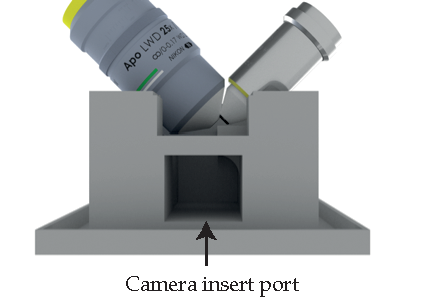
\includegraphics{./chamber_side}
         \caption{}
         \label{fig:chamber_side}
    \end{subfigure}
    \begin{subfigure}[b]{0.4\linewidth}
             \centering
        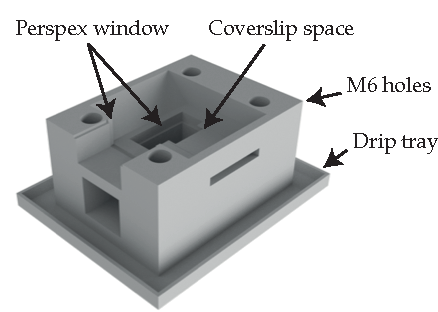
\includegraphics{./chamber_top}
         \caption{}
         \label{fig:chamber_top}
    \end{subfigure}
    \begin{subfigure}[b]{0.4\linewidth}
             \centering
        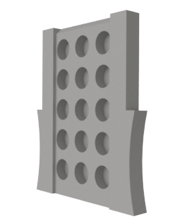
\includegraphics{./chamber_slide}
         \caption{}
         \label{fig:chamber_slide}
    \end{subfigure}
    \caption{CAD model of proposed sample chamber, featuring modular heater inserts with magnet cut-out tray.
    On the side of the chamber and below the sample, Perspex windows are inserted and sealed using cyanoacrylate (Super-Glue), this ensures a liquid-tight seal.}
\end{figure}

On the side of the chamber and below the sample, Perspex windows are inserted and sealed using cyanoacrylate (Super-Glue), this ensures a liquid-tight seal.
The adhesive is applied whilst the surface protective film is on the Perspex and removed only when the cyanoacrylate is fully set as vapour cyanoacrylate settles on surfaces and is causes opacity.
A secondary window should be cut and inserted facing the user for sample positioning, in the same manner.
This allows both objectives to be accurately positioned with respect to the mounted sample by eye, fine correction can then be achieved using texture in the sample either from bright-field or fluorescence modes.

The sample window below not only allows for a small camera module (Pi-cam, Raspberry P) to be positioned.
The camera chosen here allows for the attachment of a supplemental light source (Pi Cam) with infrared and white light illumination.
The under-sample illumination is useful for the positioning of samples without laser illumination, minimising overall photon dose.
Users may also find the additional illumination modes valuable when coarse positioning using a camera on the low magnification illumination arm.
For this system, the illumination arm is a \SI{10}{\times} objective versus the detection magnification of \SI{25}{\times}\SI{1.25}{\times}, and so coarse positioning is made along the illumination objective.

The camera model chosen here, uses a very short focal distance lens which is matched to the height of void below the where the sample is mounted in the sample chamber.
It is also compatible with the \emph{Bright-PI} which offers sufficiently bright field illumination as well as an IR modality which could be used provided the user insert the correction filters in their detection paths.

To protect the delicate objectives from crashing into a sharp edge of the cover-glass, the sample chamber is chamfered along it edges parallel to the objectives.
The chamfers serve to minimise liquid within the imaging area.
This decreases the cost per experiment as well as mitigating any significant spillage.
At the bottom of the sample chamber an additional drip tray is incorporated prevent spillage from overfill of immersion medium.
For cellular imaging, the entire assembly may be immersed in Isopropanol or Virkon for several minutes, and supplemented with sterilising if required.
Ubiquitous biologically inert plastics used in 3D printing are ABS and PLA; we note that ABS and PLA 3D printed chambers do not survive autoclaving nor overnight washes with Vircon or IPA.
If the chamber is exposed to severe imaging conditions that require containment, multiple chambers may be printed and disposed; allowing for high-throughput imaging when compared to a machined chamber which would require sterilisation after each use.
The design features cleared M6 holes to mount the chamber to a breadboard below, in this case the chamber is attached to a breadboard insert on the XY translation stage (Prior  H101F).
Other spacings and sizings of mounting holes may be easily added to the chamber on an ad-hoc basis using common 3D CAD packages (Autodesk Inventor, SolidWorks, OpenScad).

% The adhesive is applied whilst the surface protective film is on the Perspex and removed only when the cyanoacrylate is fully set as vapour cyanoacrylate settles on surfaces and is causes opacity.
% A secondary window should be cut and inserted facing the user for sample positioning, in the same manner.
% This allows both objectives to be brought with good accuracy to the mounted sample by eye alone, fine correction can then be achieved using texture in the sample either from brightfield or fluorescence modes.
% The sample window below not only allows for a pi-cam to be positioned, but can also be used in conjunction with the Bright-pi, a pi cam add-on which illuminates the camera’s subject with both infrared and white LED light.
% The under-sample illumination is useful for positioning of embryos without laser illumination along the detection path.
% Users may also find the additional illumination modes valuable when coarse positioning using a camera on the illumination arm of the system too as Illumination objectives typically have a lower magnification than their detection counter parts in high NA light-sheet systems.
% A raspberry-pi module should be used as it’s focal distance is matched to the height of the attached CAD model as well as it’s compatibility with the Bright-PI which offers sufficiently bright field illumination as well as an IR modality which could be used provided the user insert the correction filters in their infinity space.

\begin{figure}
    \centering
    \begin{subfigure}[b]{0.45\linewidth}
    \centering
    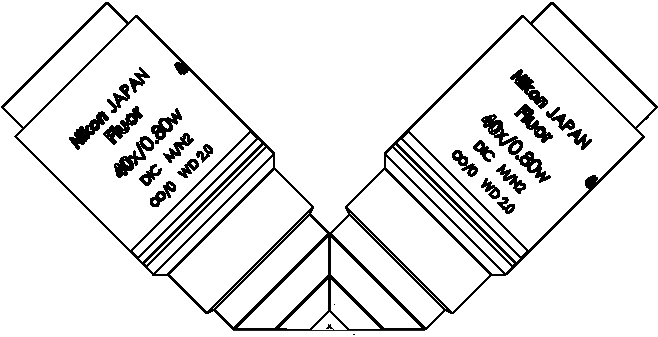
\includegraphics[width=0.9\linewidth]{./matched_objectives}
    \caption{}
    \end{subfigure}
    \begin{subfigure}[b]{0.45\linewidth}
        \centering
        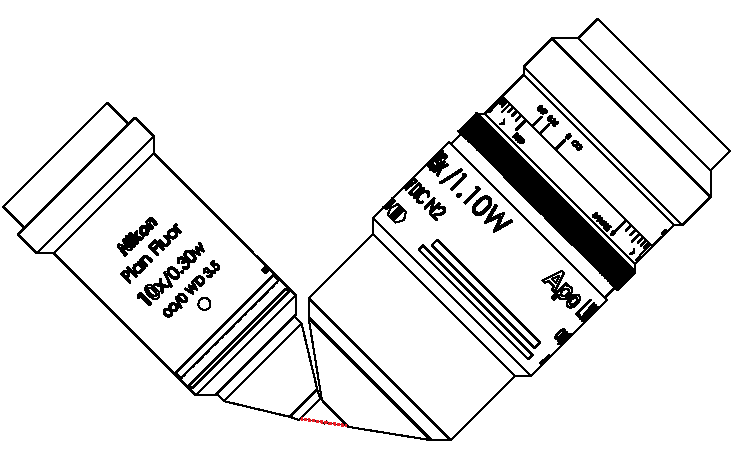
\includegraphics[width=0.9\linewidth]{./assymetric_nikon}
        \caption{}
    \end{subfigure}
    \caption{
    a) Shows the objective arrangement as found in the diSPIM, whereby each imaging arm is computationally fused to create a final image volume with higher axial resolution, from the two views.
    b) Shows the objective combination from the Lattice light-sheet where the detection objective is very high NA
    }
    \label{}
\end{figure}

% Figure 2.
% Possible large NA objective combinations using the proposed sample chamber design
% To minimise imaging medium and protect the delicate objectives from crashing into a sharp edge of the cover-glass, the sample chamber is chamfered along it edges parallel to the objectives.
% The chamfers make the chamber fail safe as well as serving to minimise liquid within the imaging area.
% This minimises the cost per experiment as well as mitigating any significant spillage.
% At the bottom of the sample chamber an additional drip tray is augmented should a leak spring or a user overfills immersion medium.
% For cellular imaging, the entire assembly may be immersed in Isopropanol or Virkon for several minutes, and supplemented with sterilising if required.
% ABS and PLA 3D printed chambers do not survive autoclaving nor overnight washes with Vircon or IPA.
% If the chamber is exposed to severe imaging conditions that require containment, multiple chambers may be printed and disposed; allowing for high-throughput imaging when compared to a machined chamber which would require sterilisation after each use.
% The design features M6 cleared holes to mount the chamber to a breadboard below, in this case the chamber is attached to a breadboard insert on a Prior Stage [which stage].
% Other spacing’s and sizing’s of mounting holes may be added to the chamber on an ad-hoc basis.

\begin{figure}
    \centering
    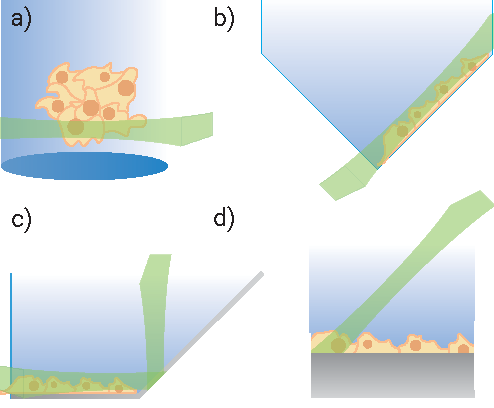
\includegraphics{./mounting_straegies_cells}
    \caption{Strategies for mounting cell culture.
    a) shows a cylinder of MatriGel used to scaffold a 3D cell culture.
    b) Shows cells cultured on a cuvette with the illumination arriving through the orthogonal flat window.
    c) shows a reflective cuvette being used to redirect a concomitant illumination and detection into orthogonal, similar reflection strategies exist such as mounting small mirrors to a single objective or positioning small mirrors carefully near the sample.
    d) shows cells cultured on a small pedestal and imaged using an iSPIM configuration, difficulties arise in keeping such pedestals sterile during incubation and then attaching to the system whilst submerged.
    }
    \label{fig:mounting_straegies_cells}
\end{figure}

\begin{figure}
    \centering
    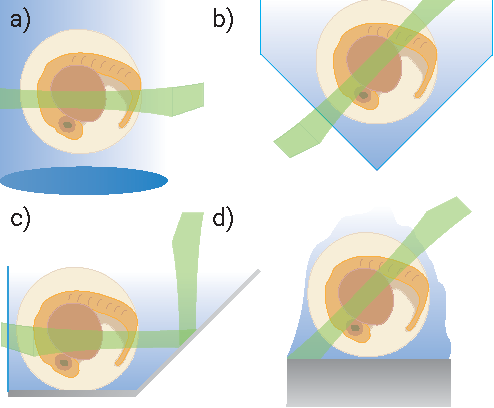
\includegraphics{./mounting_straegies_fish_cartoon}
    \caption{Strategies for mounting Zebrafish are shown.
    a) uses a cylinder of agarose suspended from above and lowered into the imaging volume;
    b) is a cuvette whereby the flat windows are imaged and excited through orthogonally;
    c) has a small pedestal with a small amount of agarose placed on top, the entire system is submerged in medium to match refractive indices.}
    \label{fig:mounting_straegies_fish}
\end{figure}

\section{Method}

Zebrafish (see Figure 3) were dechorionated manually with tweezers using a stereo-microscope on a bed of agarose, immersed in embryo medium.
The dechorionated Zebrafish were then transferred into molten agarose and gently drawn into a length of FEP attached to a pipette tip.
Organisms may be mounted agarose within in FEP tubing to help match refractive indices between water immersion medium and the agarose.
0.8\% agarose VII was used, higher percentage agarose may restrict the growth of a developing embryo as well as cause more scattering and RI mismatch; agarose VII produces the best imaging conditions of the agarose\cite{4}.
Once an embryo is embedded in its agarose tubing it may be transported conveniently, for imaging; it should then be adhered to a \SI{25}{\milli\metre\square} coverslip using colourless nail varnish at each end of the tubing whilst avoiding the active imaging area along the FEP tubing.
For cell culture imaging SHSY5Y neuronal cells were cultured of on coverglass that had been functionalised with poly-l-lysene to help cell adhesion.
In Figure \ref{fig:cell_image} cells were fixed using formaldehyde and imaged in phosphate-buffered saline (PBS).
For live cell studies a medium without phenol red and that does not require atmospheric control should be used (ex. HEPES).


% Zebrafish (see Figure 2) were dechorionated manually with tweezers using a stereo-microscope on a bed of agarose, immersed in embryo medium.
% The dechorionated Zebrafish were then transferred into molten agarose and gently drawn into a length of FEP attached to a pipette tip.
% Organisms may be mounted agarose within in FEP tubing to help match refractive indices between water immersion medium and the agarose.
% 0.8% agarose VII was used, higher percentage agarose may restrict the growth of a developing embryo as well as cause more scattering and RI mismatch; agarose VII produces the best imaging conditions of the agarose3.
% Once an embryo is embedded in its agarose tubing it may be transported conveniently, for imaging; it should then be adhered to a 25 mm2 coverslip using nail varnish at each end of the tubing whilst avoiding the activate imaging area along the FEP tubing.
% For cell culture imaging SHSY5Y neuronal cells were cultured of on coverglass that had been functionalised with Poly-L-lysene to help cell adhesion.
% For the image in Figure 3 cells were fixed using Formaldehyde and imaged in Phosphate-buffered saline (PBS).
% For live cell studies a medium without Phenol red and that does not require atmospheric control should be used (ex.
% HEPES).

\subsection{Sample Positioning}

Samples mounted on coverslips were held in the chamber using a magnetically positioned bar.
Pre-warmed immersion medium was added slowly and filled to 3mm below the top of the chamber.
The entire chamber was then driven below the objective pair by eye and carefully raised.
Lateral positioning is best achieved by matching eye level with the sample and adjusting the stage as required.
Axial positioning is best coarsely adjusted by driving the sample slightly away from the laser illumination so as to not harm the sample.
The scattered spot on the immersion-medium-glass interface should be minimised by eye.
Finally, the sample chamber should be moved laterally again until a fluorescent signal on the camera can be detected.
The secondary raspberry pi-cam below may also be used as an additional positioning camera.
This is more useful for embryos as the coarse adjustment method as above can be challenging due to their transparency even with guiding marks on the coverglass.
When considering very large samples or samples that over large areas, multiple images may need to be stitched together creating a mosaic.
For the objective pair as used here, the sample chamber allows for \SI{2}{\milli\metre} by \SI{10}{\milli\metre} lateral and \SI{1}{\milli\metre} axial movement.
For systems with Piezo objective scanners, the mosaicking of volumes may drastically reduce the overall time acquisition of a mosaicked volume by requiring fewer overall steps.
Both approaches are available for the design presented here, provided care is taken to set hard limits on where the sample chamber is driven to.


% Samples mounted on coverslips were held in the chamber using a magnetically positioned bar.
% Pre-warmed immersion medium was added slowly and filled to 3mm below the top of the chamber.
% The entire chamber was then driven below the objective pair by eye and carefully raised.
% Lateral positioning is best achieved by matching eye level with the sample and adjusting the stage as required.
% Axial positioning is best coarsely adjusted by driving the sample slightly away from the laser illumination so as to not harm the sample.
% The scattered spot on the immersion-medium-glass interface should be minimised by eye.
% Finally, the sample chamber should be moved laterally again until a fluorescent signal on the camera can be detected.
% The secondary raspberry pi-cam below may also be used as an additional positioning camera.
% This is more useful for embryos as the coarse adjustment method as above can be challenging due to their transparency even with guiding marks on the coverglass.
% Depending on the system configuration, imaging may require the movement of the sample chamber.
% For the objective pair as used here, this allows for 2mm by 10mm lateral and 1mm axial movement [CHECK NUMBERS].
% For systems with Piezo objective scanners, a hybrid technique of objective scanning and volumetric mosaicing provides a fast method for large area scanning incurring fewer stitching errors compared to full sample mechanical scanning.


\begin{figure}
    \centering
    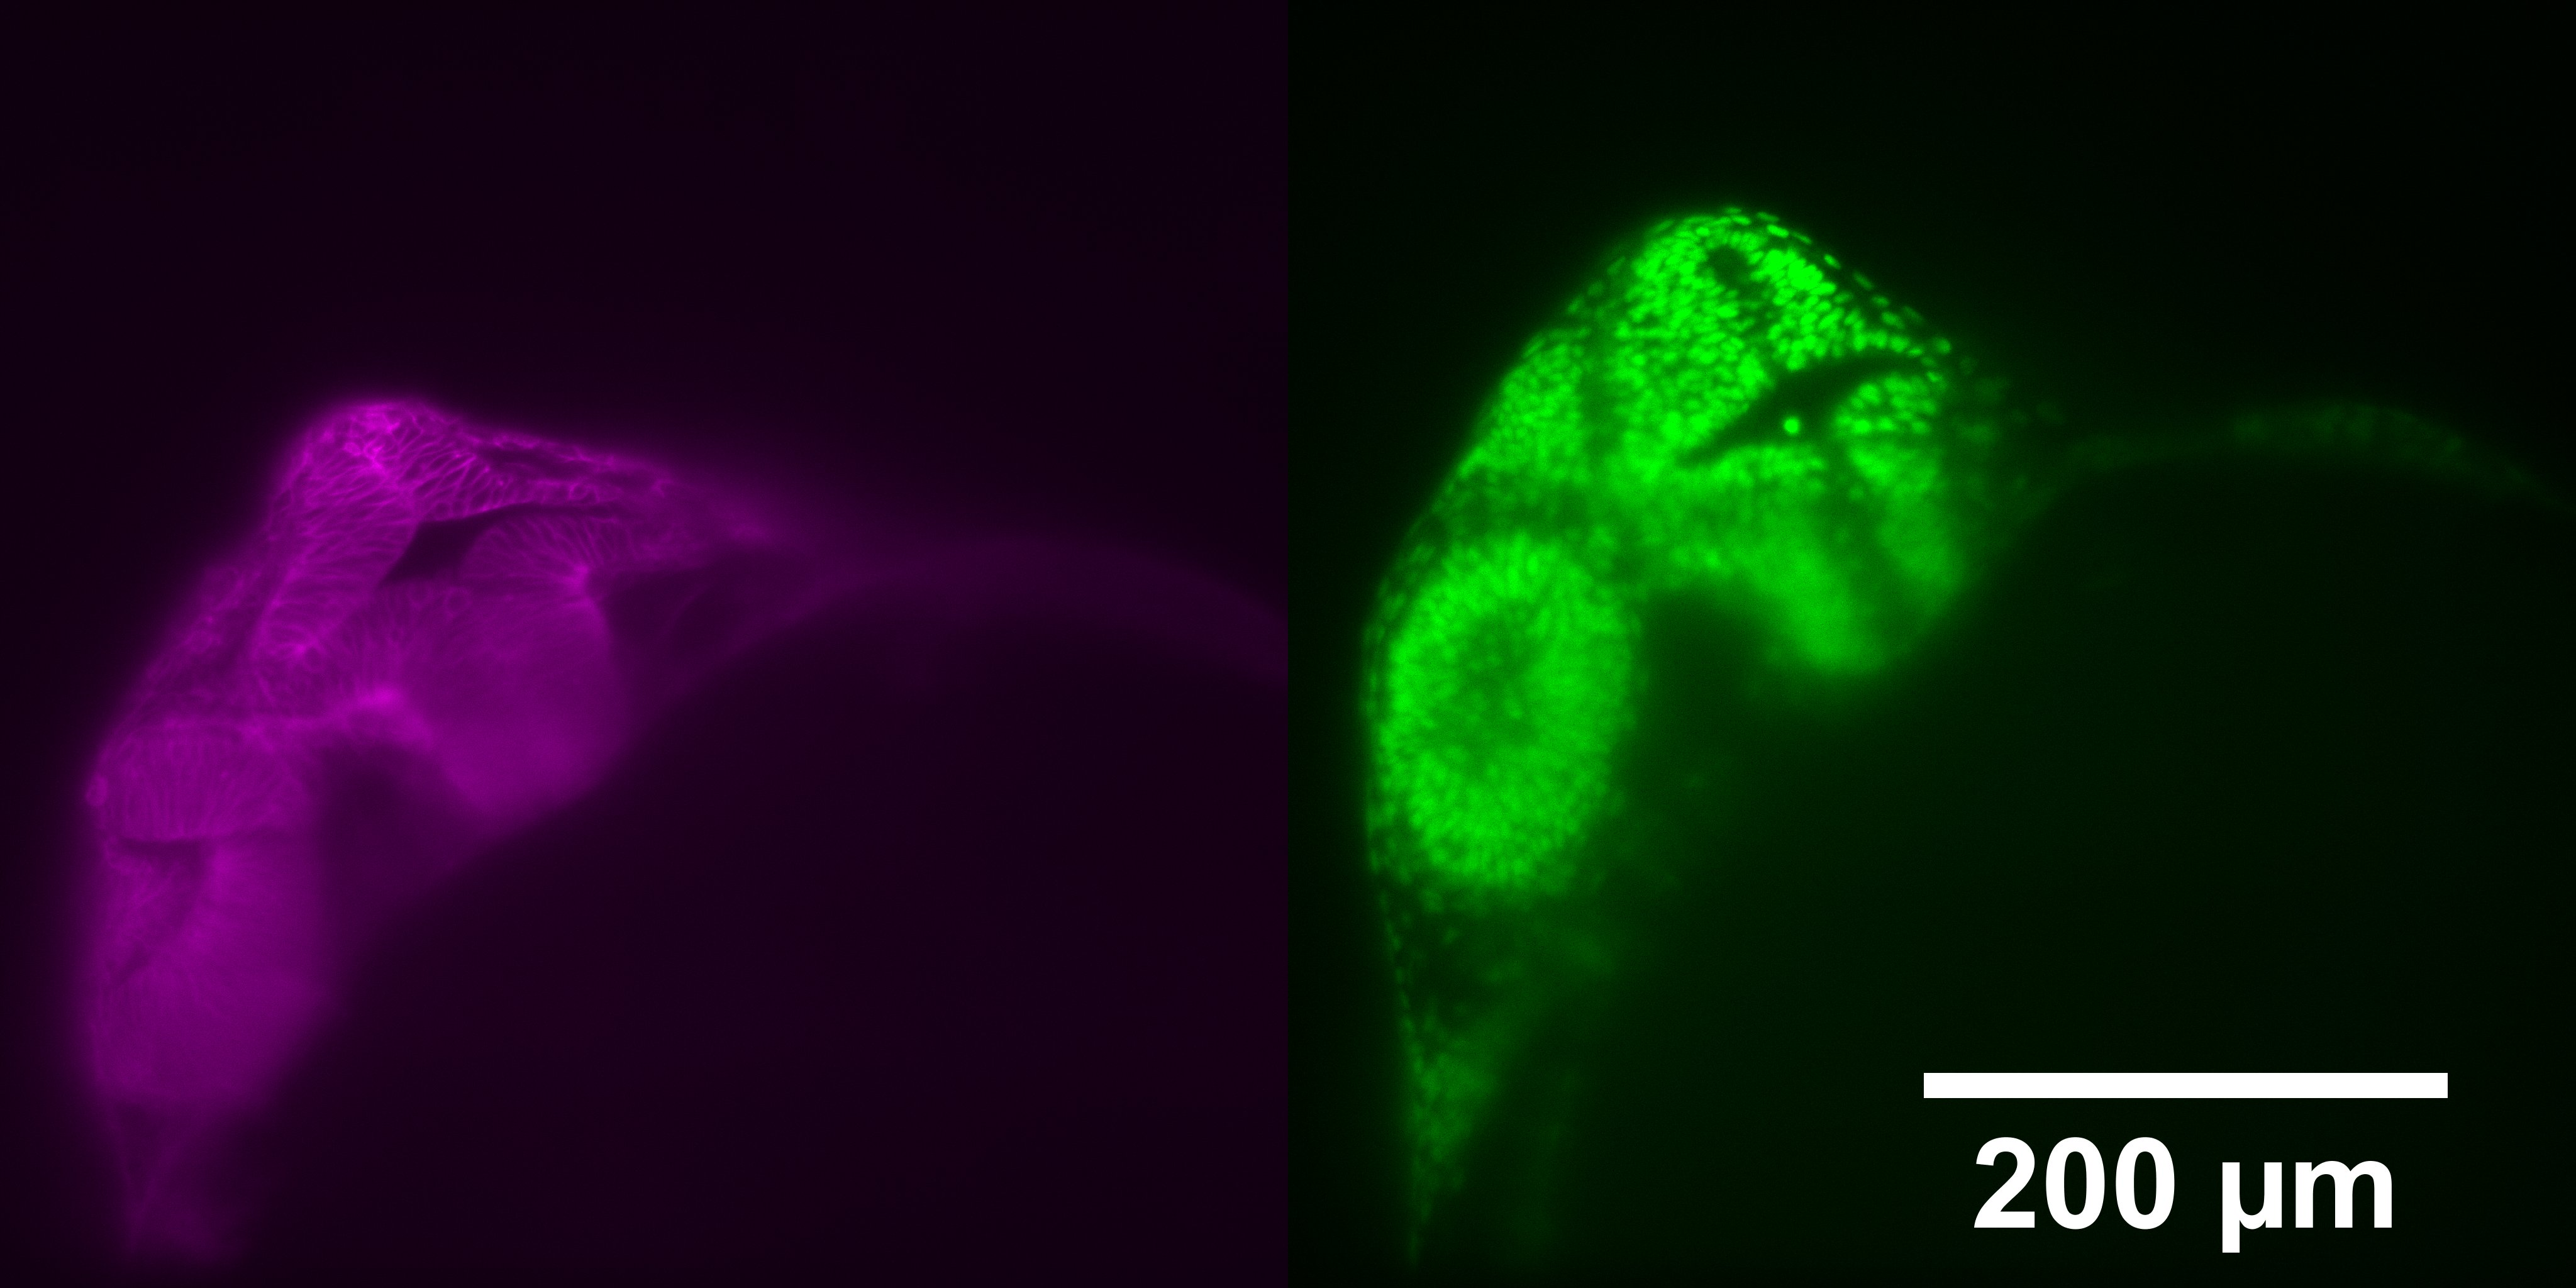
\includegraphics[width=0.8\linewidth]{./fish_image}
    \caption{Two colour imaging of a transgenic Zebrafish 24 h.p.f.
    The left hand image shows a membrane-local  Beta-actin: mcherryCAAX probe;
    the right image shows fluorescent histones within the nucleus using a h2b:gfp probe.}
    \label{fig:fish_image}
\end{figure}

\begin{figure}
    \centering
    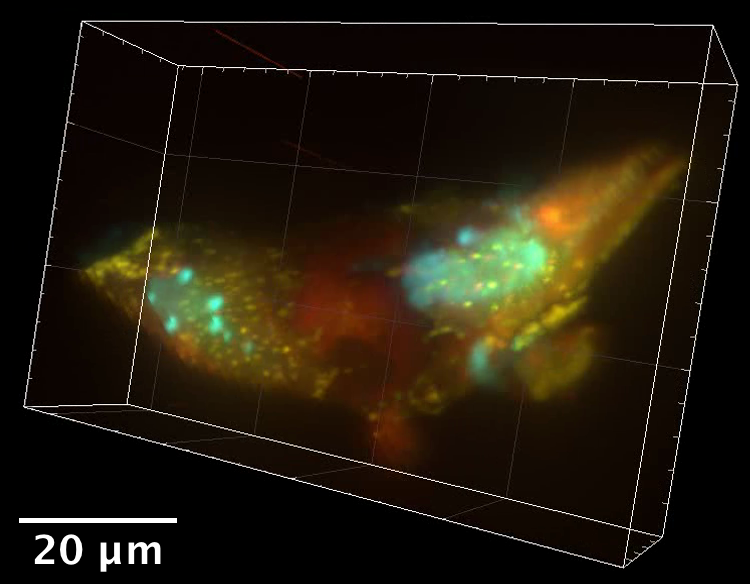
\includegraphics[width=0.8\linewidth]{./cell_image}
    \caption{A three-colour composite 3D image, as rendered in Imaris, of a pair of SHSY5Y cells.}
    \label{fig:cell_image}
\end{figure}

\section{Remarks}

We have presented an open hardware solution to address the challenge of mounting a breadth of biological samples in a high NA inverted light-sheet system.
The principles behind the design can be  used directly, applied and extended and provide a robust starting point which can be easily modified for an end user’s needs.
Using a single piece of 3D printed material means the unit is robust as it has no moving parts; disposable; sterile and mass producible.
The unique design also allows for a large volume of travel allowing for volumetric mosaicking and medium-throughput imaging.
The device features many useful features such as a sample mounting camera below, a Perspex window for safe positioning, multiple safety features and sample heating.
Future models of this design could also include atmospheric control for long time-lapse imaging of cell cultures.
Such a sample chamber may also be used for other biologicals on the same scale as cells to embryos, potentially including the imaging of organoids.

% We have presented an open hardware solution to address the challenge of mounting a breadth of biological samples in a high NA inverted light-sheet system.
% The principles behind the design can be applied and extended to other systems with ease.
% Using a single piece of 3D printed material means the unit is robust as it has no moving parts; disposable; sterile and mass producible.
% The unique design also allows for a large volume of travel allowing for volumetric mosaicing and medium-throughput imaging.
% The device features many useful features such as a sample mounting camera below, a Perspex window for safe positioning, multiple safety features and sample heating.
% Future models of this design could also include atmospheric control for long time-lapse imaging of cell cultures. Such a sample chamber may also be used for other biologicals on the same scale as cells to embryos, this includes the imaging of organoids though none have been used in this work.
%


%Agarose stuff
%http://what-when-how.com/molecular-biology/agarose-molecular-biology/
